%%=============================================================================
%% Methodologie
%%=============================================================================

\chapter{\IfLanguageName{dutch}{Methodologie}{Methodology}}
\label{ch:methodologie}

%% TODO: Hoe ben je te werk gegaan? Verdeel je onderzoek in grote fasen, en
%% licht in elke fase toe welke stappen je gevolgd hebt. Verantwoord waarom je
%% op deze manier te werk gegaan bent. Je moet kunnen aantonen dat je de best
%% mogelijke manier toegepast hebt om een antwoord te vinden op de
%% onderzoeksvraag.

% \lipsum[21-25]


\section{Overzicht}

\subsection{Installatie en indeling}

\subsubsection{Installatie}

Het aanmaken van een nieuwe applicatie in Angular, React en Mithril verloopt in alle drie de gevallen tamelijk vlot. Hoewel er bij Mithril meer handelingen nodig zijn, verloopt het toch vlotter dan Angular en React die in slechts twee commands een applicatie kunnen maken. Figuur \ref{fig:setups} toont de nodige commands om een applicatie aan te maken en te laten uitvoeren.  Angular en React zijn al volledig geconfigureerd. Echter bij Mithril zijn er extra handelingen vereist voordat de applicatie uitgevoerd kan worden:

\begin{itemize}
    \item In het \texttt{package.json} bestand moet er een \texttt{start} entry toegevoegd worden aan het \texttt{scripts} object. Hoe dit object er uit moet zien, kan gevonden worden in figuur \ref{fig:mithril-package-json}.
    \item Er moet een \texttt{src/index.js} bestand aangemaakt worden. Om te starten met een ''Hello World'' kan de code uit figuur \ref{fig:mithril-index-js} gebruikt worden.
    \item Als laatste moet er een \texttt{index.html} gecreëerd worden. Hoe de HTML er uit moet zien, kan gevonden worden in figuur \ref{fig:mithril-index-html}.
    \item Daarna kan \texttt{index.html} geopend worden in de browser om het resultaat te kunnen bekijken.
\end{itemize}

\begin{figure}[!ht]
    \subfloat[Angular setup\label{subfig-1:angular-setup}]{%
        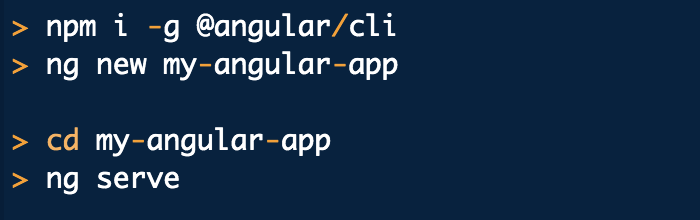
\includegraphics[width=0.3\textwidth]{Angular-setup.png}
    }
    \hfill
    \subfloat[React setup\label{subfig-2:react-setup}]{%
        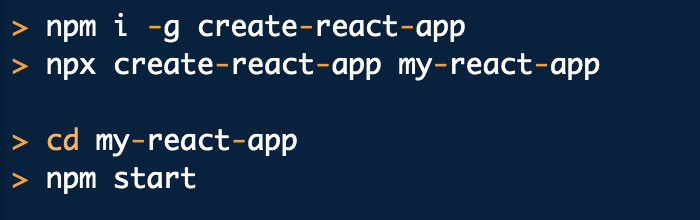
\includegraphics[width=0.3\textwidth]{React-setup.png}
    }
    \hfill
    \subfloat[Mithril setup \label{subfig-3:mithril-setup}]{%
        
\includegraphics[width=0.3\textwidth]{Mithril-setup.png}
    }
    \caption{De nodige commands om een nieuwe applicatie op te zetten.}
    \label{fig:setups}
\end{figure}

\begin{figure}
    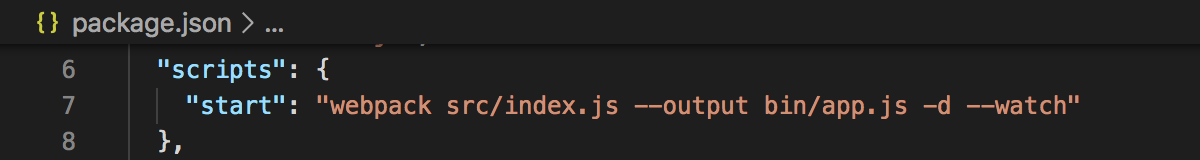
\includegraphics[width=\textwidth]{./img/Mithril-package-json.png}
    \caption{De \texttt{start} entry in het \texttt{scripts} object binnen \texttt{package.json}.}
    \label{fig:mithril-package-json}
\end{figure}

\begin{figure}
    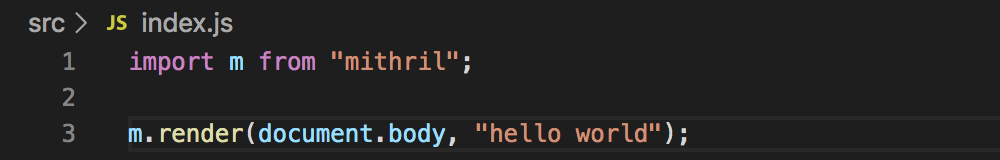
\includegraphics[width=\textwidth]{./img/Mithril-index-js.png}
    \caption{De code nodig binnen het \texttt{src/index.js} bestand om 'hello world' weer te geven.}
    \label{fig:mithril-index-js}
\end{figure}

\begin{figure}
    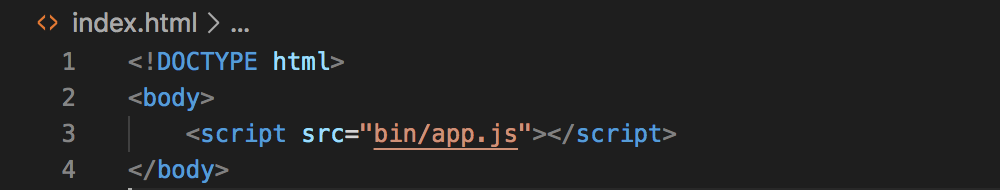
\includegraphics[width=\textwidth]{./img/Mithril-index-html.png}
    \caption{De HTML binnen het \texttt{index.html} bestand.}
    \label{fig:mithril-index-html}
\end{figure}

\subsubsection{Indeling}

Nadat de applicaties aangemaakt zijn, kan gekeken worden naar de structuur die Angular, React en Mithril hanteren. Dit is belangrijk om het standpunt van alle drie de technologieën te achterhalen.

Bij het bekijken van de architectuur die gebruikt wordt in Angular applicaties, is het duidelijk dat Angular zijn folderstructuur baseert op de componenten binnen de applicatie. Binnen de \texttt{src} folder die Angular zelf aanmaakte zit er een \texttt{app} folder die een basis module en component bevat. De module bestaat uit een bestand \texttt{app.module.ts}, terwijl de component uit vier bestanden bestaat zoals getoond in figuur \ref{subfig-1:angular-structuur}. Deze bestanden zijn:
\begin{itemize}
    \item app.component.css
    \item app.component.html
    \item app.component.spec.ts
    \item app.component.ts
\end{itemize}

React daarentegen heeft geen \texttt{out-of-the-box} structuur buiten de \texttt{src} folder. Zoals figuur \ref{subfig-2:react-structuur} aantoont bevat die folder de volgende bestanden:
\begin{itemize}
    \item App.css
    \item App.js
    \item App.test.js
    \item index.css
    \item index.js
    \item logo.cvg
    \item serviceWorker.js
    \item setupTests.js
\end{itemize}

Het is duidelijk dat Mithril geen structuur bevat aangezien de \texttt{src} folder tijdens de setup van de applicatie zelf aangemaakt moet worden. Mithril's architectuur ziet er dan uit zoals figuur \ref{subfig-3:mithril-structuur} aantoont.

\begin{figure}[!ht]
    \subfloat[Angular\label{subfig-1:angular-structuur}]{%
        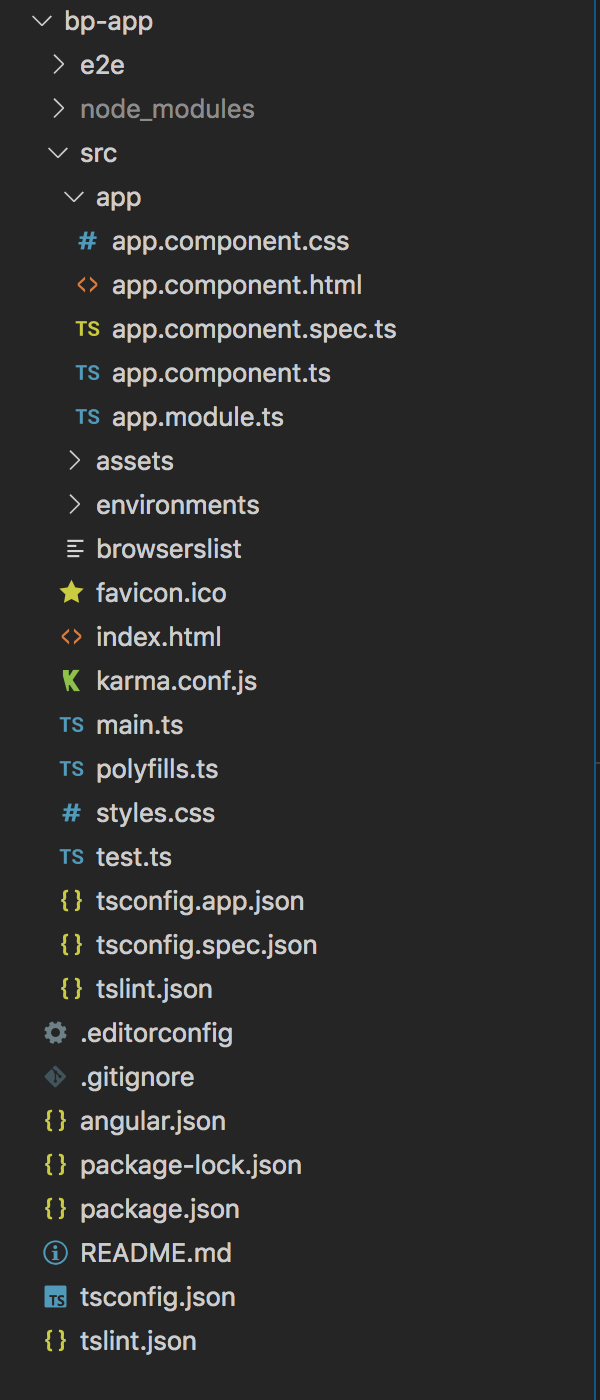
\includegraphics[width=0.3\textwidth]{Angular-structuur.png}
    }
    \hfill
    \subfloat[React\label{subfig-2:react-structuur}]{%
        
\includegraphics[width=0.3\textwidth]{React-structuur.png}
    }
    \hfill
    \subfloat[Mithril\label{subfig-3:mithril-structuur}]{%
        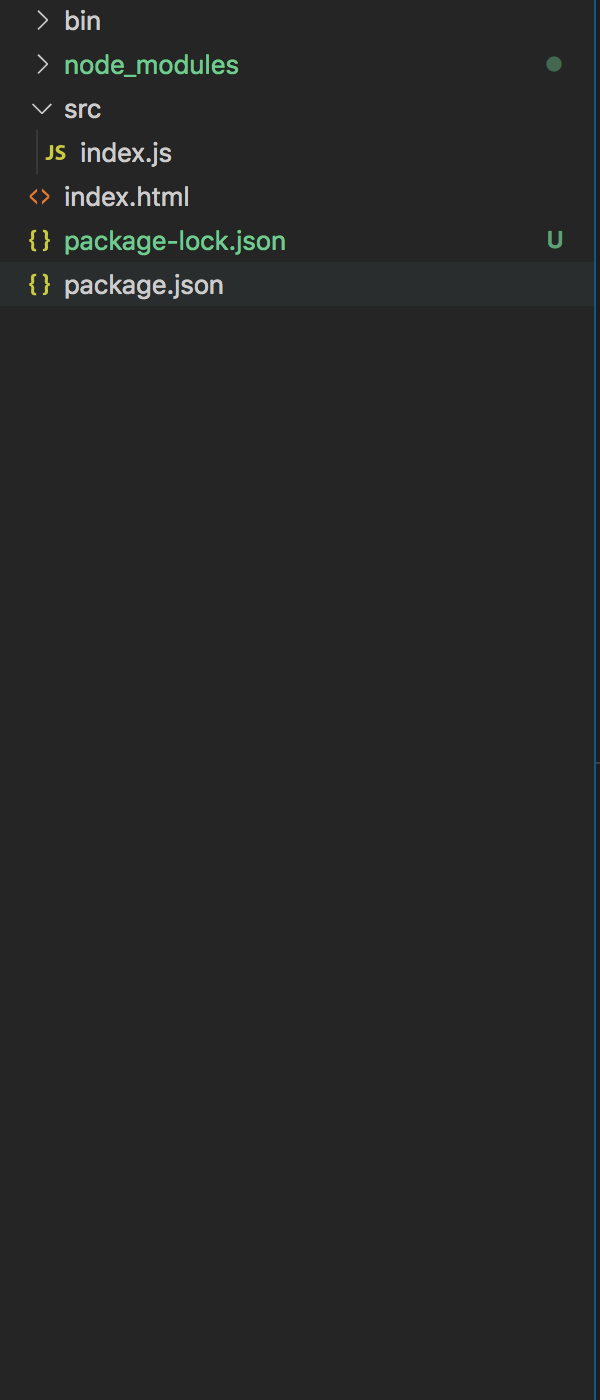
\includegraphics[width=0.3\textwidth]{Mithril-structuur.png}
    }
    \caption{De architecturen na het opzetten van een nieuwe applicatie.}
    \label{fig:structuren}
\end{figure}

\subsection{Grootte}

De grootte van de bestanden in een applicatie is belangrijk. JavaScript code moet gedownloaded worden voordat de applicatie volledig functioneel is. Hoe meer code er is, hoe langer het zal duren om de applicatie uitgevoerd kan worden. Dat beïnvloedt de responsiviteit die de gebruiker waarneemt en dat is heel belangrijk. De downloads hebben ook invloed op het verbruik in bandbreedte. \autocite{Coulman2015}

De grootte van het onderliggende framework is niet het enige dat telt. Het is ook belangrijk om de grootte van de code van de applicatie in overweging te brengen. Een framework kan een grote invloed hebben op de grootte van de applicatiecode. Een framework met veel uitgewerkte features staat ontwikkelaars toe om minder eigen applicatiecode te schrijven. Bij het vergelijken van grootte is de totale grootte (framework + app code) de beslissende factor. \autocite{Coulman2015}

Om de grootte te kunnen vergelijken, willen we ook hetzelfde weergeven wanneer de applicatie uitgevoerd wordt. Daarom wordt om te beginnen in alle drie de applicaties een component aangemaakt die een \texttt{h1} element weergeeft met ''Hello World!'' als inhoud. Figuur \ref{fig:hello-world} schetst die situatie.

\begin{figure}[!ht]
    \subfloat[Angular\label{subfig-1:angular-hello}]{%
        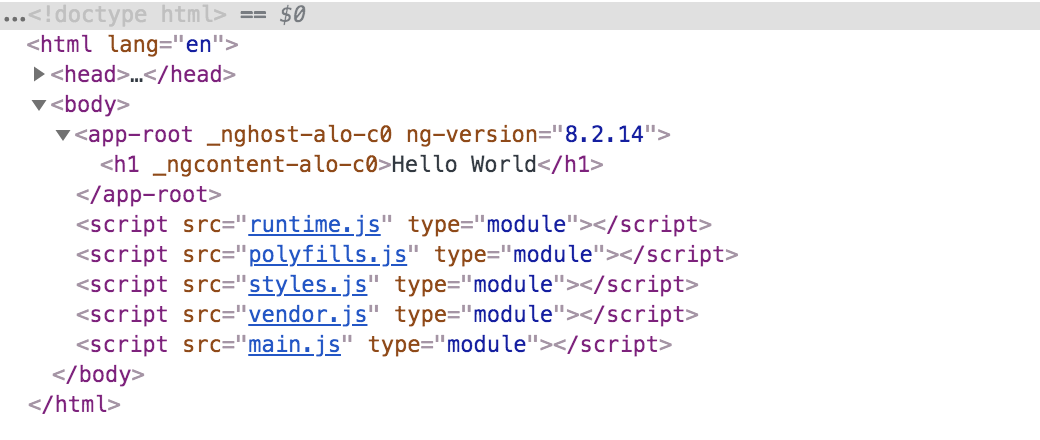
\includegraphics[width=0.3\textwidth]{Angular-hello.png}
    }
    \hfill
    \subfloat[React\label{subfig-2:react-hello}]{%
        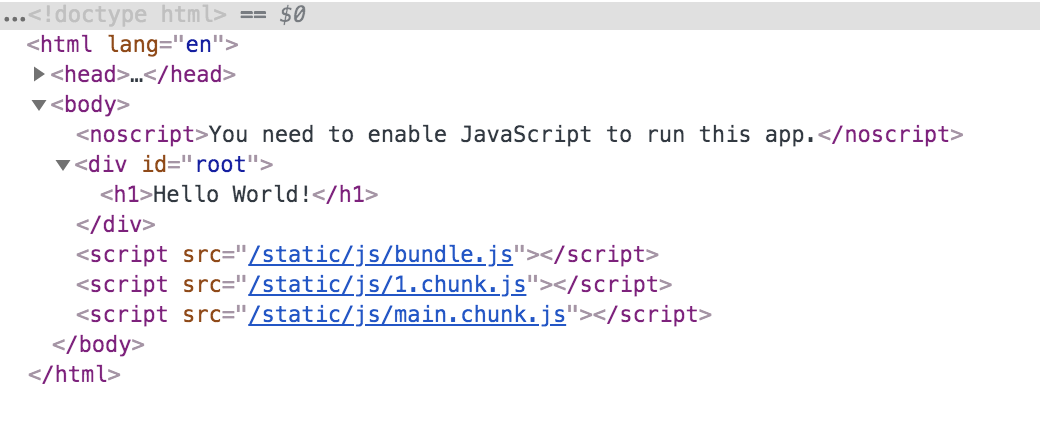
\includegraphics[width=0.3\textwidth]{React-hello.png}
    }
    \hfill
    \subfloat[Mithril\label{subfig-3:mithril-hello}]{%
        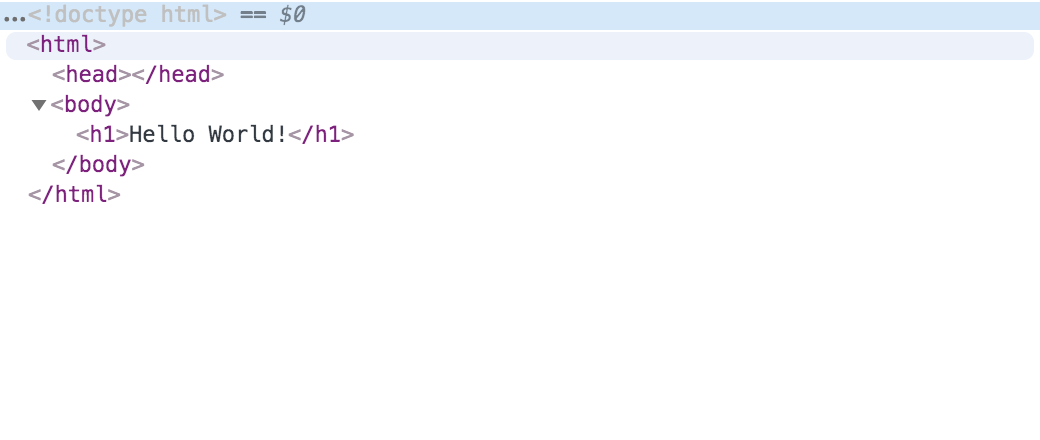
\includegraphics[width=0.3\textwidth]{Mithril-hello.png}
    }
    \caption{De ''Hello World!'' DOM-structuren nadat tekst werd weergegeven via componenten.}
    \label{fig:hello-world}
\end{figure}

Wanneer dan gekeken wordt naar de grootte van de applicaties zoals berekend in figuur \ref{fig:grootte} is het duidelijk dat Angular het meeste geheugen inneemt. React is iets kleiner in geheugenbezetting, maar Mithril steekt er met kop en schouders bovenuit als kleinste van de groep. Tabel \ref{table:grootte} geeft de benaderingen weer.

\begin{figure}
    \includegraphics[width=\textwidth]{./img/grootte.png}
    \caption{De grootte van de applicaties kan bekeken worden door het commando \texttt{du -sh *} uit te voeren.}
    \label{fig:grootte}
\end{figure}

\begin{table}
    \centering
    \begin{tabular}{|c|c|}
        \cline{2-2}
        \multicolumn{1}{c|}{} & Grootte (MB) \\ \hline
        Angular & 357 \\ \hline
        React & 245 \\ \hline
        Mithril & 61 \\ \hline
        
    \end{tabular}
    \caption{Een benaderingen van de grootte van elke ''Hello World!'' applicatie.}
    \label{table:grootte}
\end{table}

\section{Functionaliteiten}

\subsection{Componenten en templates}

In Angular, React en Mithril zijn componenten gewoon JavaScript of TypeScript klassen. Echter in React moet er een \texttt{render()} functie aanwezig zijn en in Mithril wordt een \texttt{view()} fucntie verplicht. Figuur \ref{fig:sample-components} toont hoe de componenten er uitzien. 

In Angular worden templates voorzien in een apart bestand, maar het is ook mogelijk om dit binnen het bestand van de component te doen aan de hand van het \texttt{template} attribuut voor het meta-data object van de \texttt{@Component} decorator. Figuur \ref{subfig-1:angular-sample} toont een voorbeeld van dat \texttt{template} attribuut.

React voorziet geen apart bestand, alles qua template gebeurt in de speciale \texttt{render()} functie waarin JSX geplaatst kan worden zoals in figuur \ref{subfig-2:react-sample}.

Ook in Mithril is er geen aparte template file. Alles gebeurt binnen de return van de \texttt{view()} functie. Figuur \ref{subfig-3:mithril-sample} toont hoe dat in zijn werk gaat.

\begin{figure}[!ht]
    \subfloat[Angular\label{subfig-1:angular-sample}]{%
        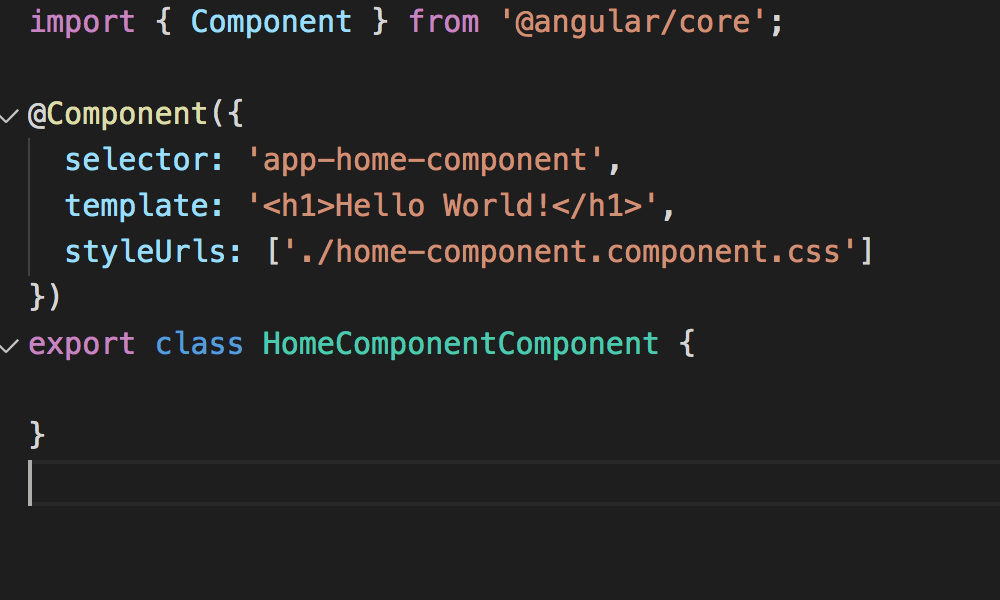
\includegraphics[width=0.3\textwidth]{Angular-component.png}
    }
    \hfill
    \subfloat[React\label{subfig-2:react-sample}]{%
        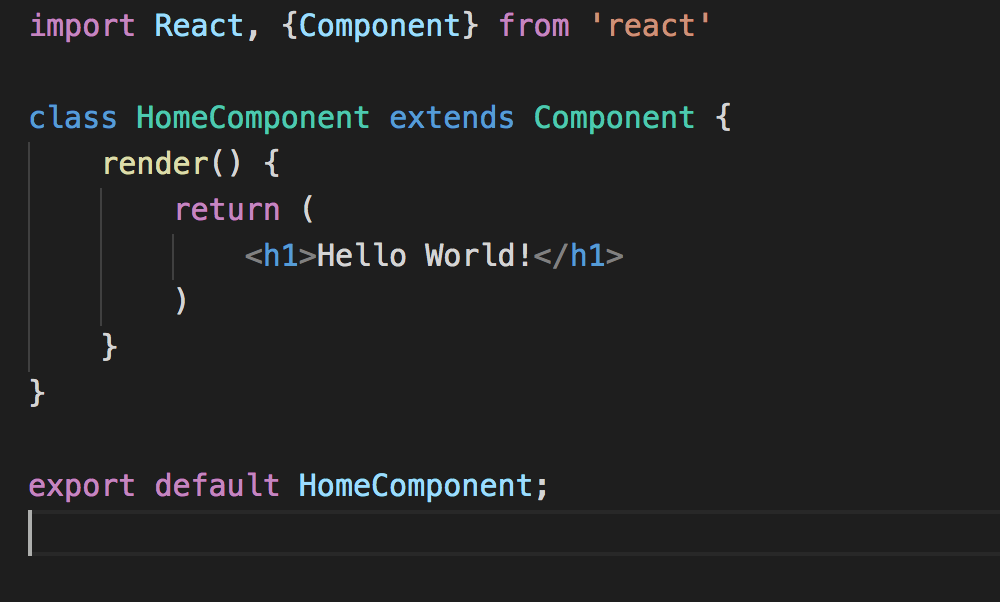
\includegraphics[width=0.3\textwidth]{React-component.png}
    }
    \hfill
    \subfloat[Mithril\label{subfig-3:mithril-sample}]{%
        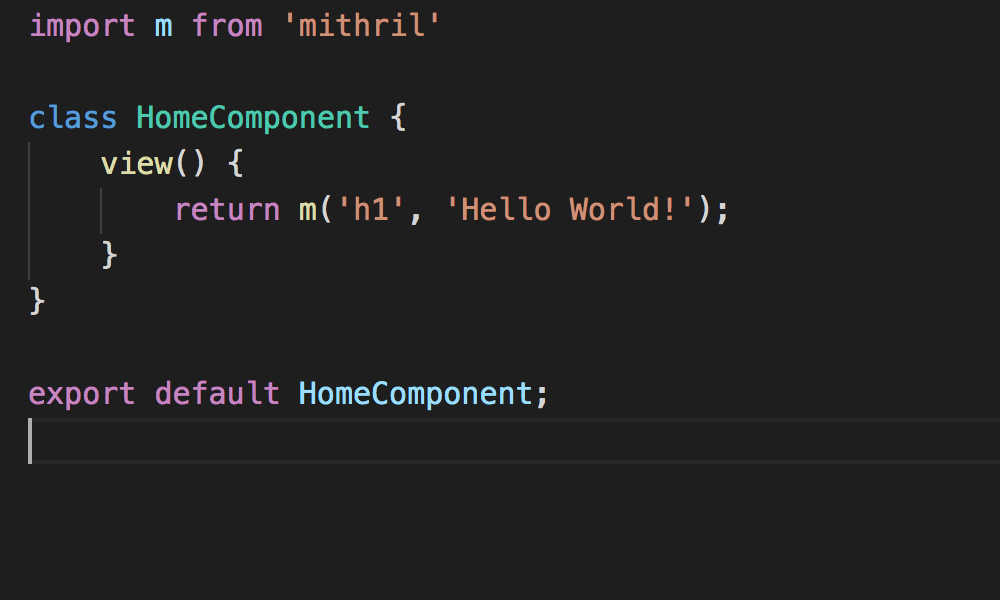
\includegraphics[width=0.3\textwidth]{Mithril-component.png}
    }
    \caption{Componenten met hun ''Hello World!'' template.}
    \label{fig:sample-components}
\end{figure}

\subsection{Prestaties}

\subsubsection{Testgevallen}

In deze bachelorproef werden enkele testgevallen onderzocht. Om een representatieve test te hebben, worden de testen 12 keer uitgevoerd waarvan de 2 meest uiteenlopende gevallen genegeerd worden. Hierdoor kan een gemiddelde bepaald worden voor 10 gevallen. De zaken die getest worden zijn als volgt: 

\begin{itemize}
    \item Het maken van 1000 componenten en deze weergeven.
    \item Het updaten van 1000 componenten en de wijziging weergeven.
    \item Het updaten van elke tiende component en de wijziging weergeven.
    \item Het verwijderen van elke tiende component en de wijziging weergeven.
    \item De startup waarbij 1000 componenten aangemaakt en weergegeven worden.
\end{itemize}

\subsubsection{Technische aspecten}

Om een duidelijk zicht te krijgen op welke technologie sneller is voor een bepaald geval, is het aan te raden om deze testen meerdere keren uit te voeren. Hierbij is het echter noodzakelijk om een referentiepunt te hebben. Om de snelheid van een testgeval te bepalen werd er gekozen om als startpunt het begin van het DOM event te nemen en als eindpunt het einde van de paint. 

Omdat er geen gemakkelijke manieren waren om de tijdsverschillen tussen het event en de paint te automatiseren, werden de waarden manueel uit de \texttt{performance} tab van de Chrome DevTools. Hierbij werd in elke opname de timestamp genomen van het DOM event. Deze waarde werd vervolgens afgetrokken van de timestamp van de paint plus de duur van die paint. Op die manier wordt de snelheid bepaald. 

Om het geheugenverbruik te bepalen werd geopteerd om gebruik te maken van \texttt{puppeteer}, een \texttt{Node.js} bibliotheek die een \texttt{high-level API} biedt om Chrome (of Chromium) te besturen via het DevTools-Protocol. Aan de hand van een klein script kan het geheugenverbruik gemeten worden.

Alle resultaten werden in een Excel bestand geplaatst en daaruit werd het gemiddelde berekend. Met de resultaten werd dan een grafiek gemaakt.

De versies van de programmas die gebruikt werden in deze bachelorproef zijn als volgt:
\begin{itemize}
    \item Google Chrome 79.0.3945.88
    \item Visual Studio Code 1.41.1
    \item Excel 16.32
    \item Angular 8.3.21
    \item React 16.12.0
    \item Mithril 2.0.4
\end{itemize}

\subsubsection{Snelheid}

Figuur \ref{fig:snelheid-resultaten} geeft de resultaten weer. Het is vanzelfsprekend dat een lagere waarde een indicatie is voor een betere prestatie. Uit deze figuur is dus duidelijk te zien dat Mithril het snelst is in alle aspecten.

\begin{figure}[!ht]
    \subfloat[1000 componenten aanmaken\label{subfig-1:testcase1}]{%
        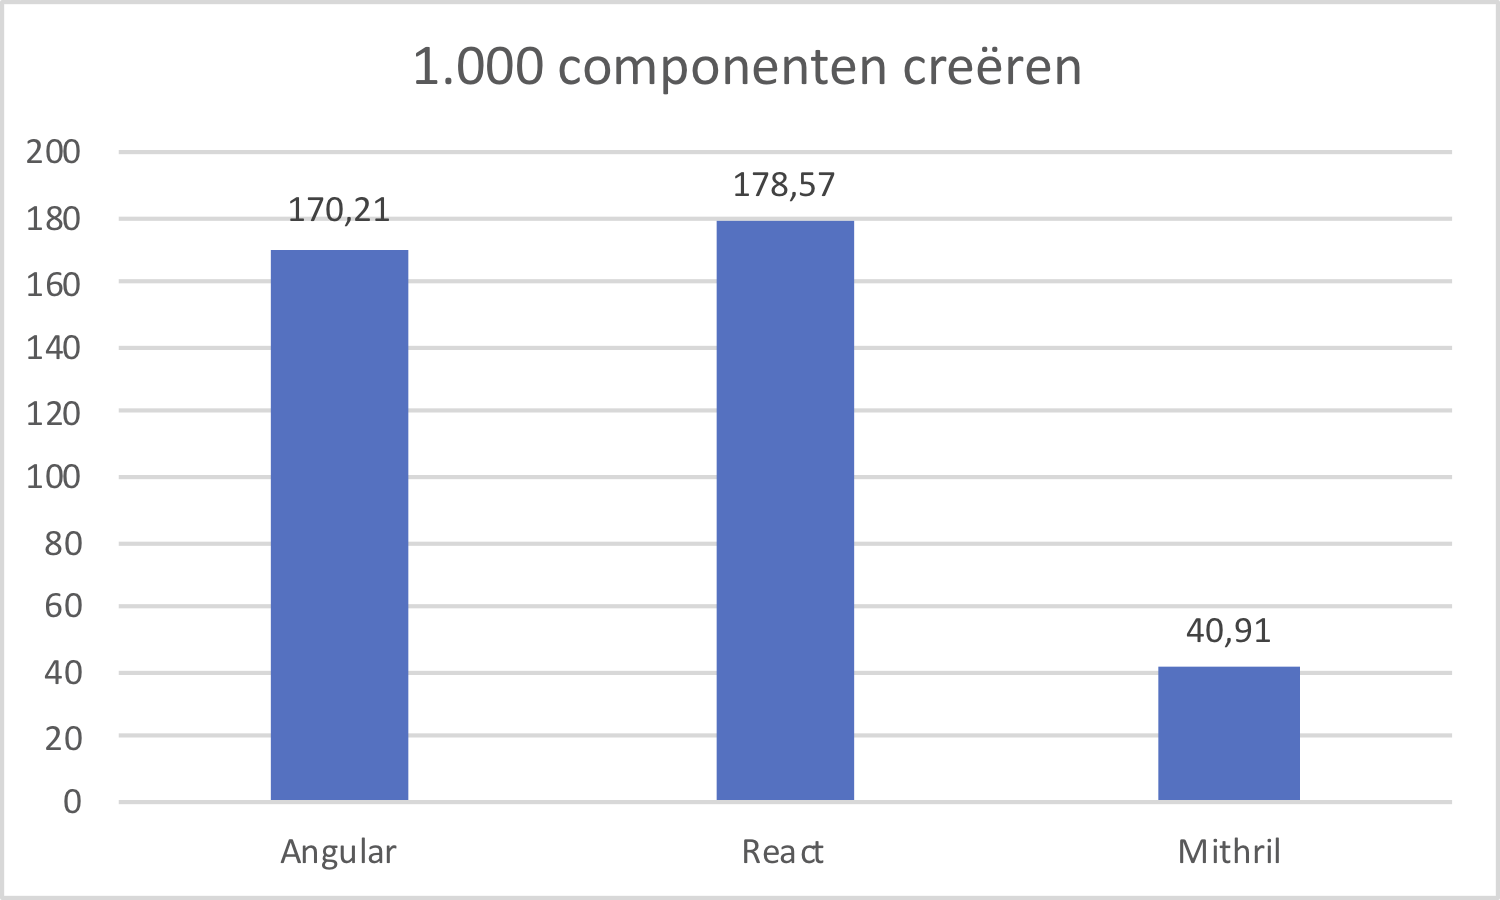
\includegraphics[width=0.45\textwidth]{testcase1.png}
    }
    \hfill
    \subfloat[1000 componenten updaten\label{subfig-2:testcase2}]{%
        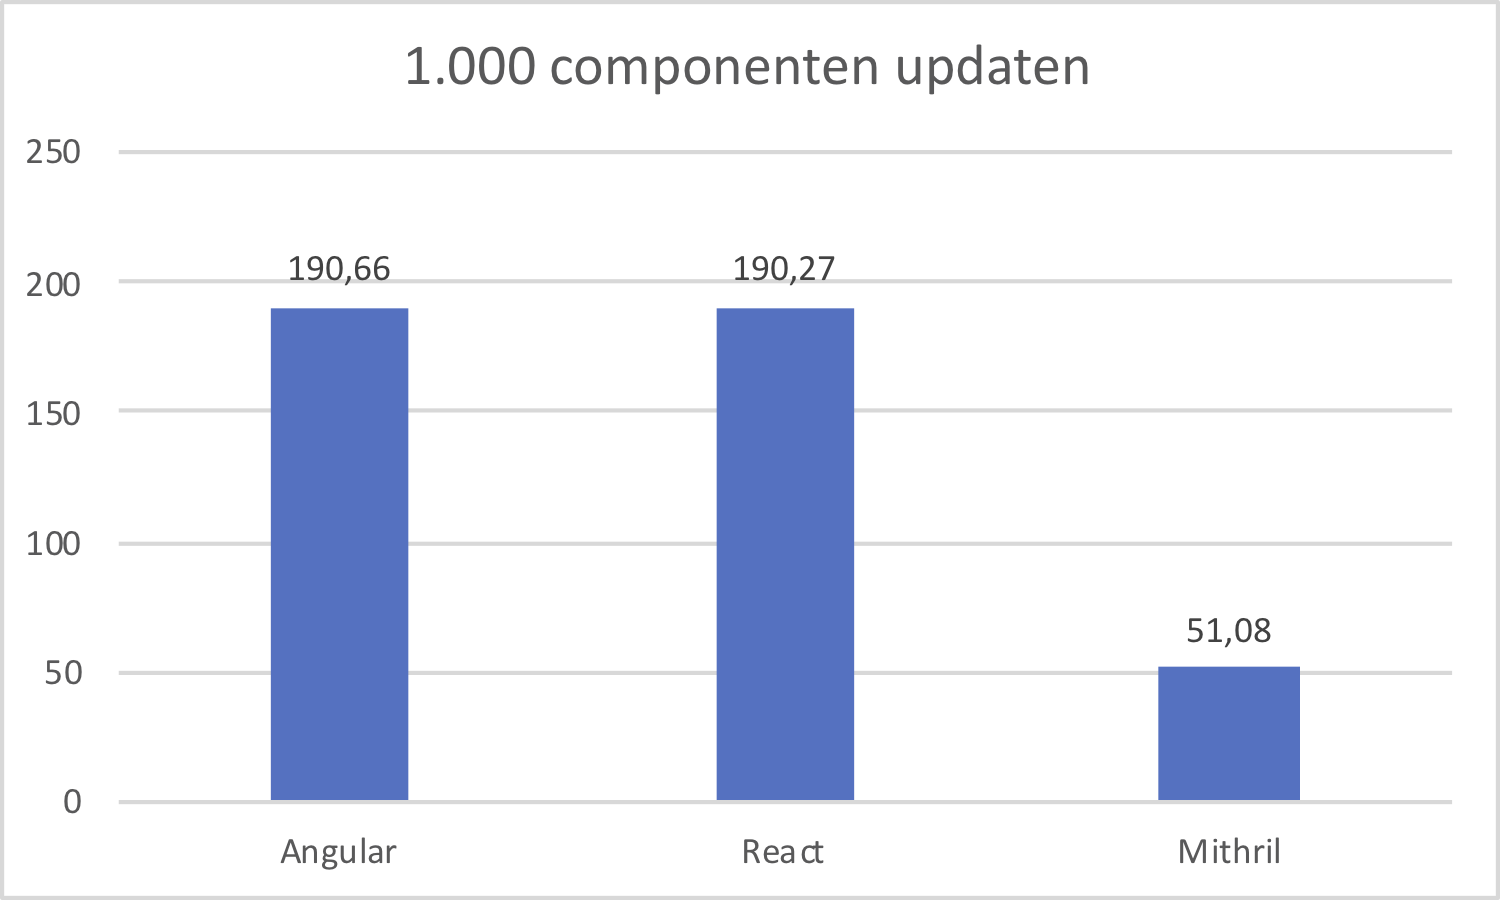
\includegraphics[width=0.45\textwidth]{testcase2.png}
    }
    \hfill
    \subfloat[Elke tiende component updaten\label{subfig-3:testcase3}]{%
        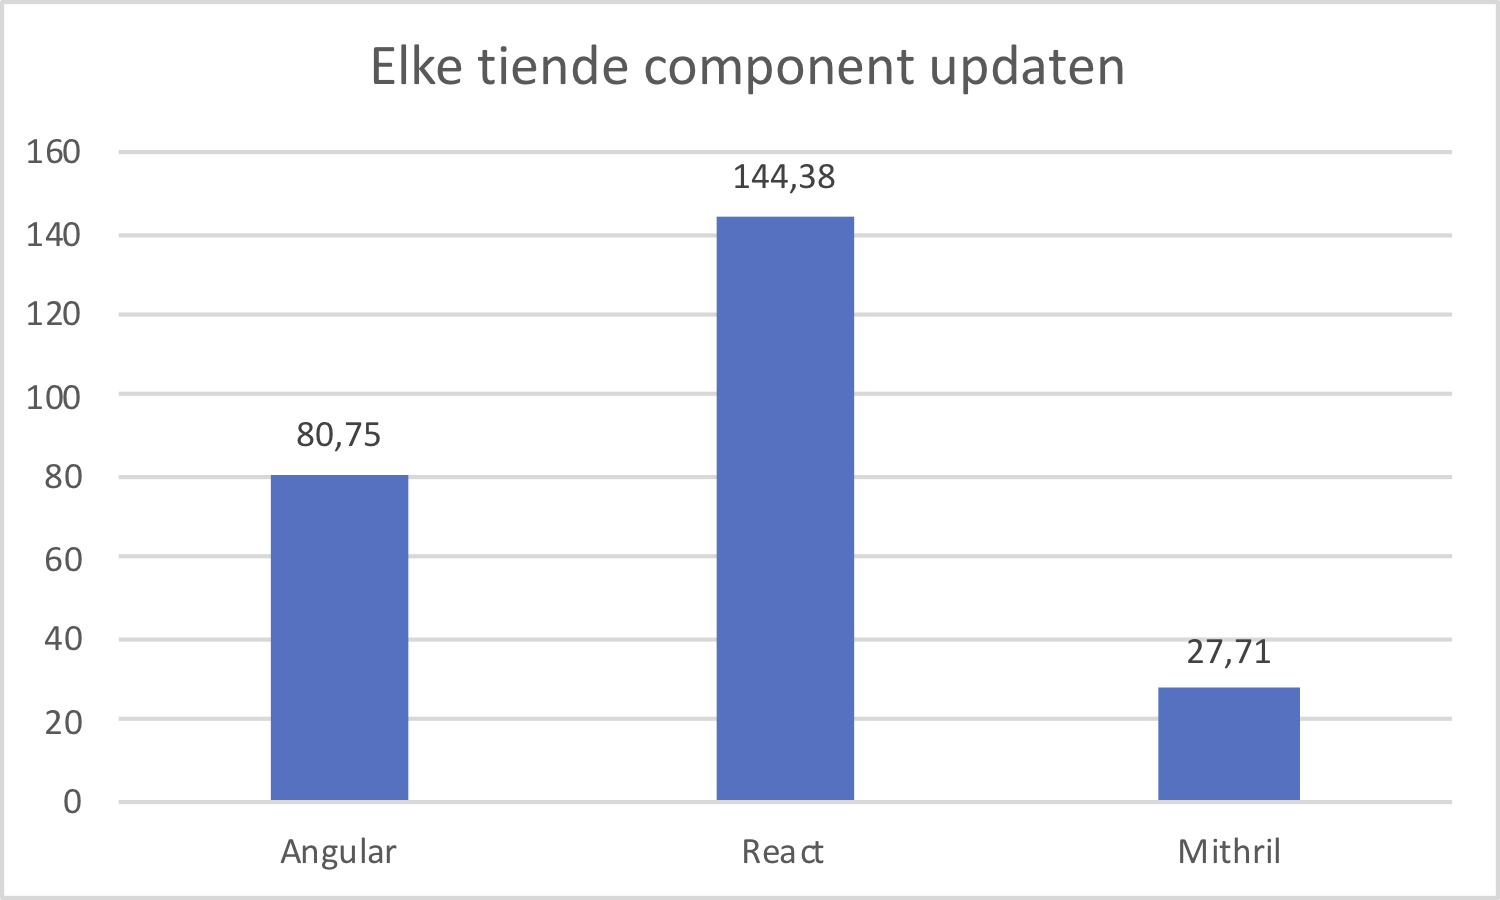
\includegraphics[width=0.45\textwidth]{testcase3.png}
    }
    \hfill
    \subfloat[Elke tiende component verwijderen\label{subfig-4:testcase4}]{%
        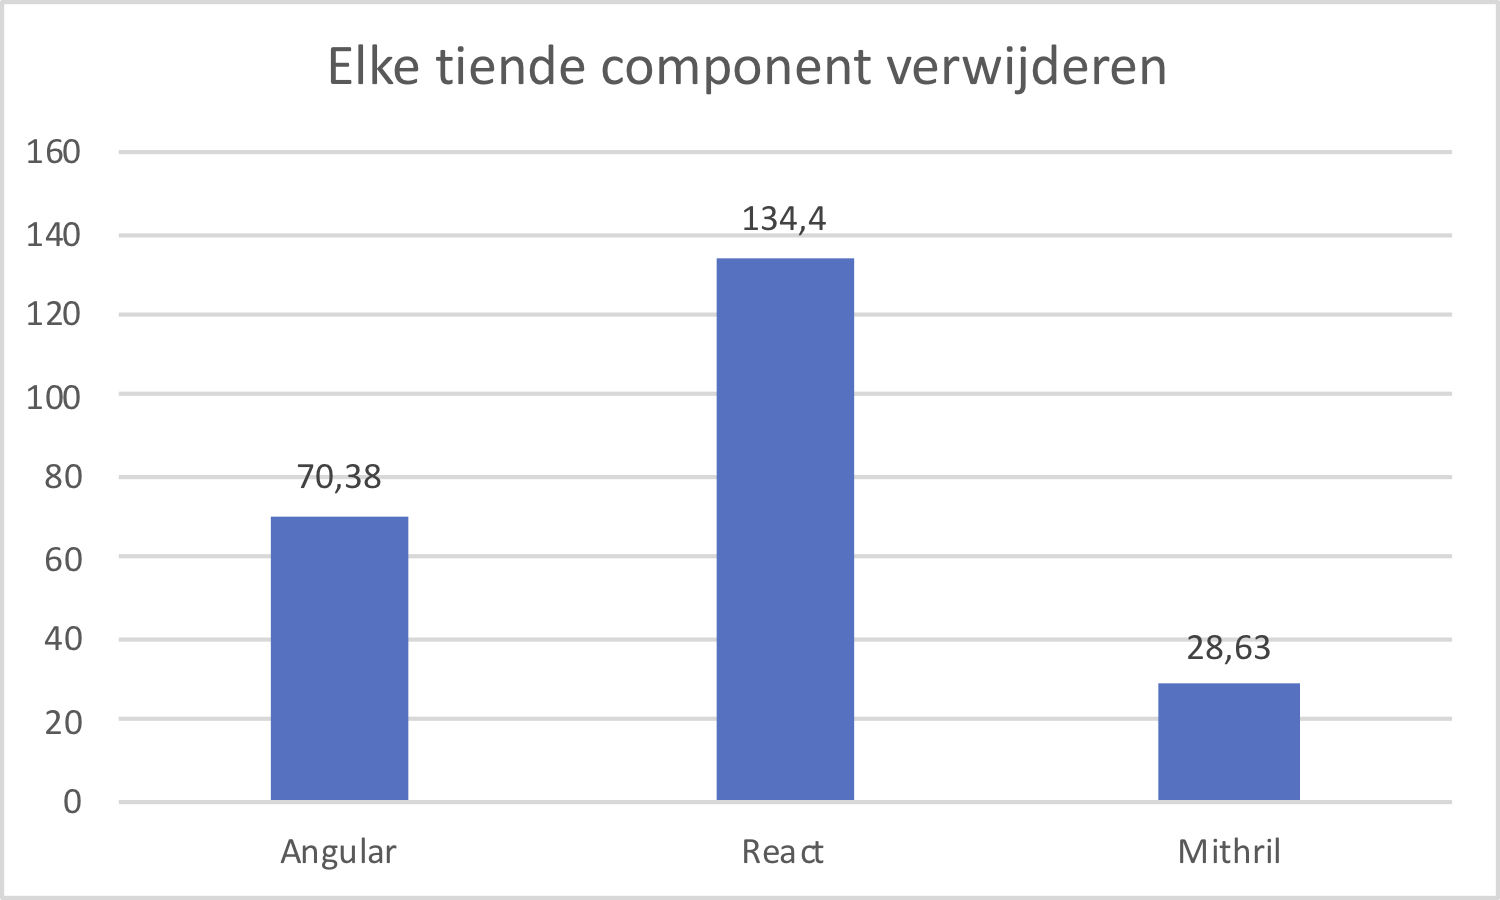
\includegraphics[width=0.45\textwidth]{testcase4.png}
    }
    \hfill
    \centering
    \subfloat[Startup + 1000 componenten aanmaken\label{subfig-5:testcase5}]{%
        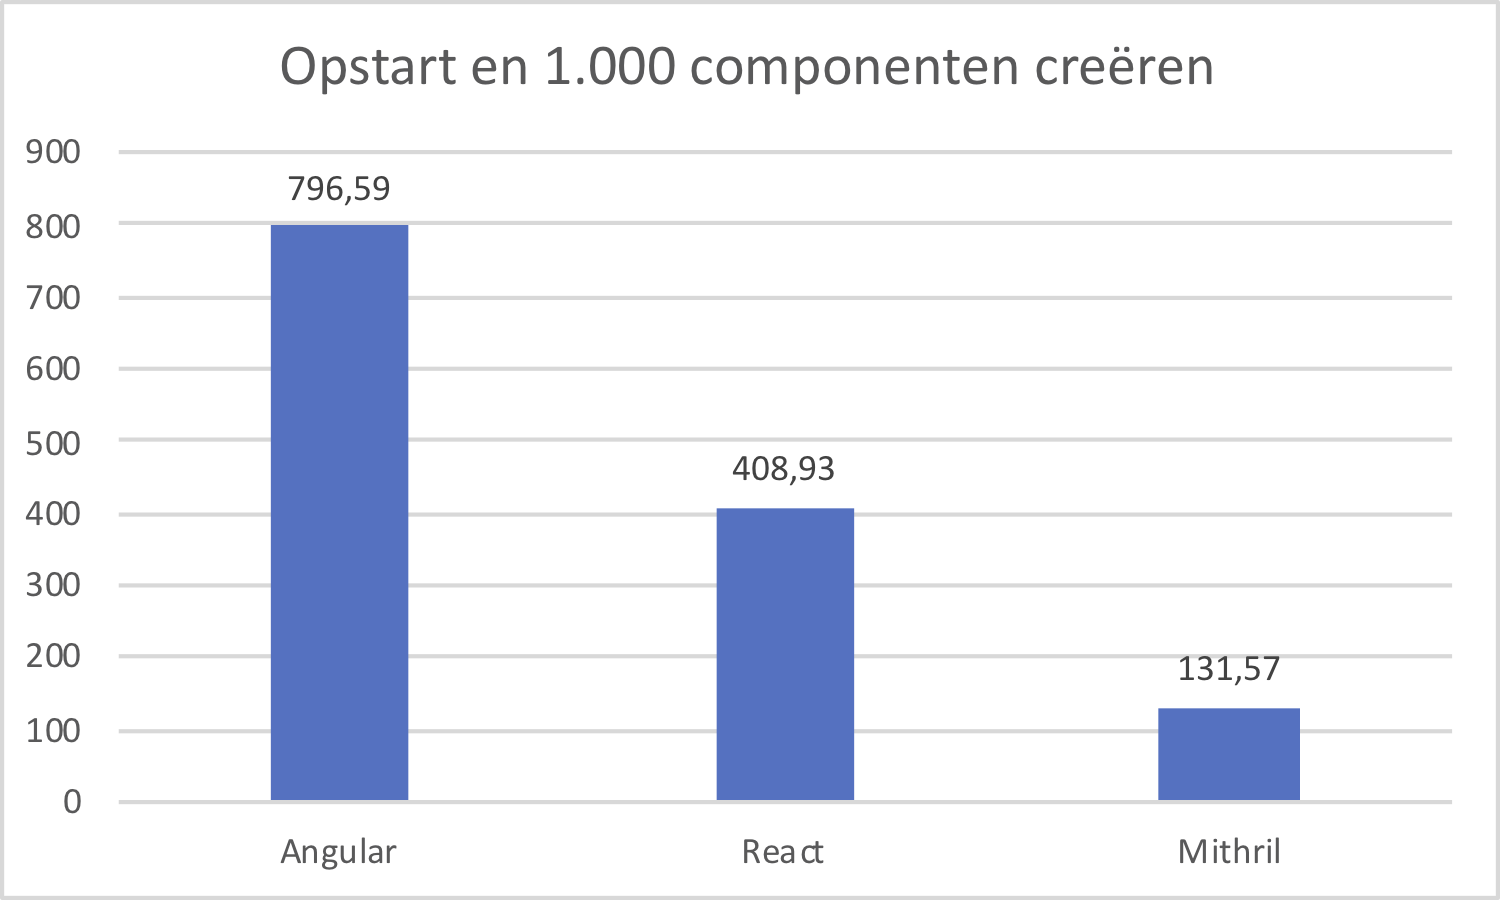
\includegraphics[width=0.45\textwidth]{testcase5.png}
    }
    \caption{Resultaten van de testen in verband met snelheid (in milliseconden).}
    \label{fig:snelheid-resultaten}
\end{figure}

\subsubsection{Geheugenverbruik}

In deze test werd gekeken naar de gebruikte hoeveelheid geheugen bij het opstarten en het maken van 1000 componenten. Hierbij werd zoals eerder vermeld gebruik gemaakt van \texttt{puppeteer}. Door een eenvoudig script te laten uitvoeren kon de \texttt{JSHeapSizeUsed} bepaald worden. Figuur \ref{fig:geheugenverbruik} toont de resultaten van dat script. Zoals duidelijk te zien is op de grafiek verbruikt Angular het meeste geheugen, terwijl Mithril het minst verbruikt.

\begin{figure}
    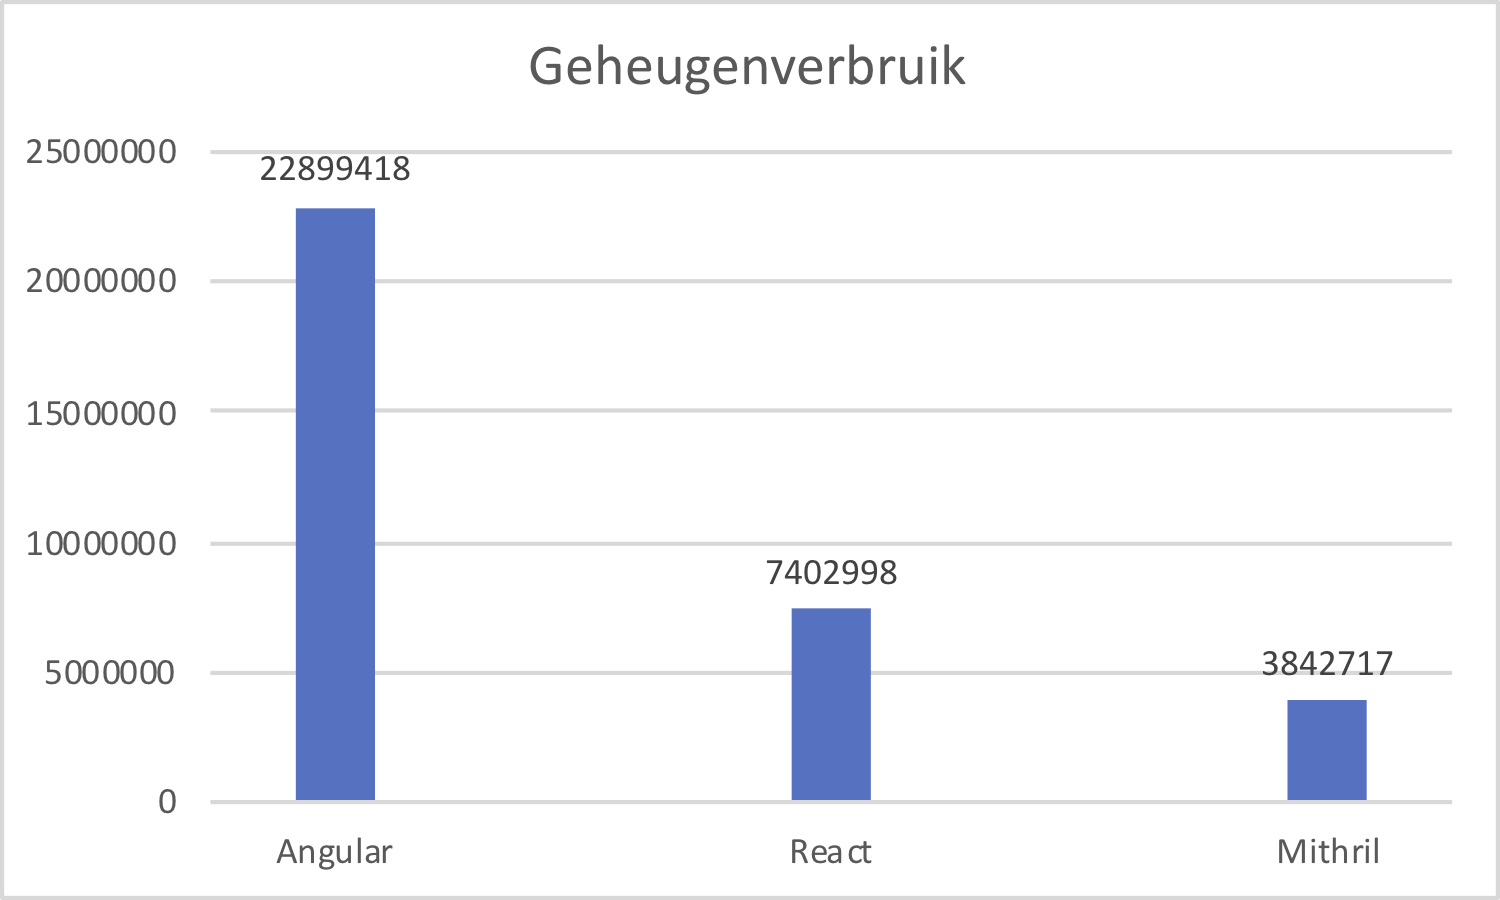
\includegraphics[width=\textwidth]{./img/geheugenverbruik.png}
    \caption{Het gemeten geheugenverbruik bij het opstarten en het creëren van 1000 componenten (in B).}
    \label{fig:geheugenverbruik}
\end{figure}

\subsection{Populariteit}

\subsubsection{Google Trends}

Als eerste wordt gekeken naar de populariteit van Angular, React en Mithril door gebruik te maken van Google Trends\footnote{https://trends.google.com/trends/explore?cat=1142\&date=2013-01-01\%202020-01-05\&q=\%2Fg\%2F11c6w0ddw9,React,Mithril}. Google Trends is een website die beheerd wordt door Google en de populariteit van de zoekopdrachten analyseert over bepaalde regio's en talen. In dit geval wordt er gekeken naar de wereldwijde interesse en werden alle talen geanalyseerd. Figuur \ref{fig:googletrends} toont de resultaten van Google Trends. Deze grafiek is relatief, het werd zo opgesteld dat het hoogste punt de waarde 100 krijgt, alle andere waarden worden afgewogen ten opzichte van dat punt. Belangrijk is hier wel dat niet alle zoekopdrachten verwijzen naar het framework of de library aangezien de namen ervan ook gewoon voorkomen in de Engelse taal of in fictieve boeken en films. Daarnaast is het ook niet mogelijk om Angular te scheiden van AngularJS, waardoor de resultaten dus niet volledig representatief zijn. Zoals op de grafiek te zien is, blijft React stevig groeien, terwijl Angular stagneert. 

\begin{figure}
    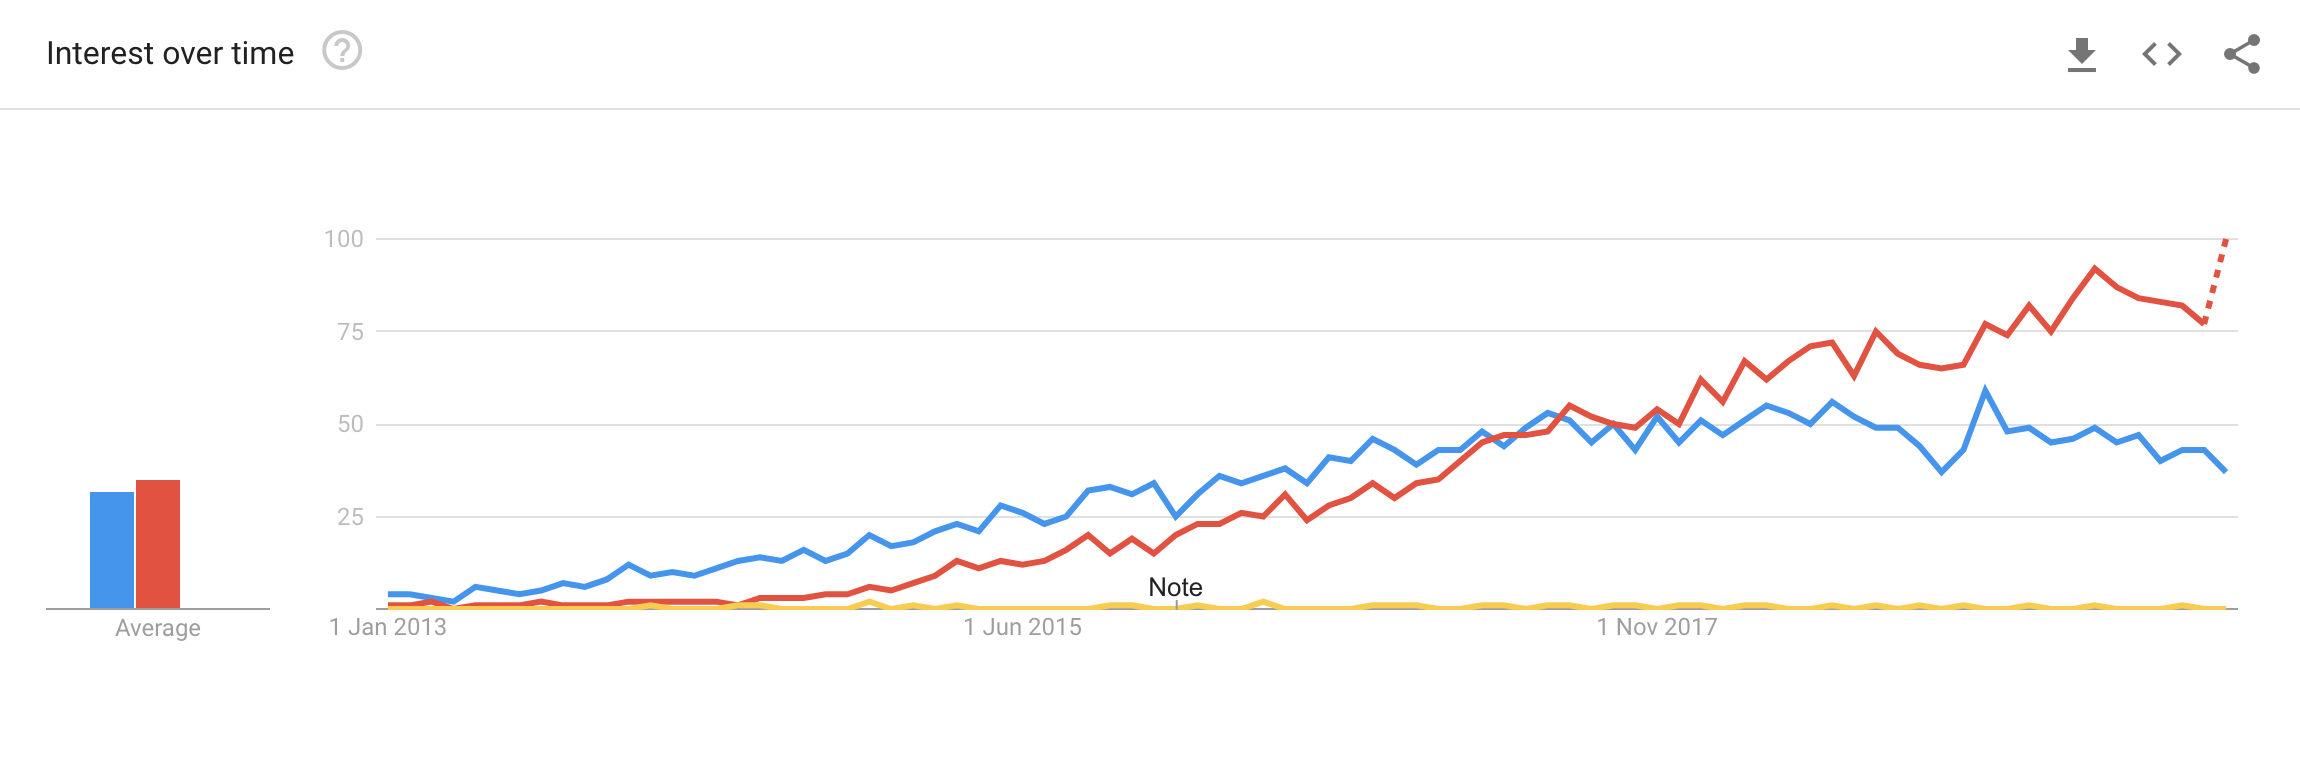
\includegraphics[width=\textwidth]{./img/googletrends.png}
    \caption{De grafiek in verband met populariteit die gegenereerd werd door Google Trends.}
    \label{fig:googletrends}
\end{figure}

\subsubsection{npm trends}

Vervolgens wordt er gekeken naar npm trends\footnote{https://www.npmtrends.com/react-vs-mithril-vs-@angular/cli}. Dit is een website die het aantal downloads analyseert vanuit npm. Figuur \ref{fig:npmtrends} geeft ongeveer hetzelfde resultaat weer als Google Trends. Ook hier is de grafiek niet 100\% representatief aangezien Angular opgedeeld is in meerdere onderdelen of deelpakketten.

\begin{figure}
    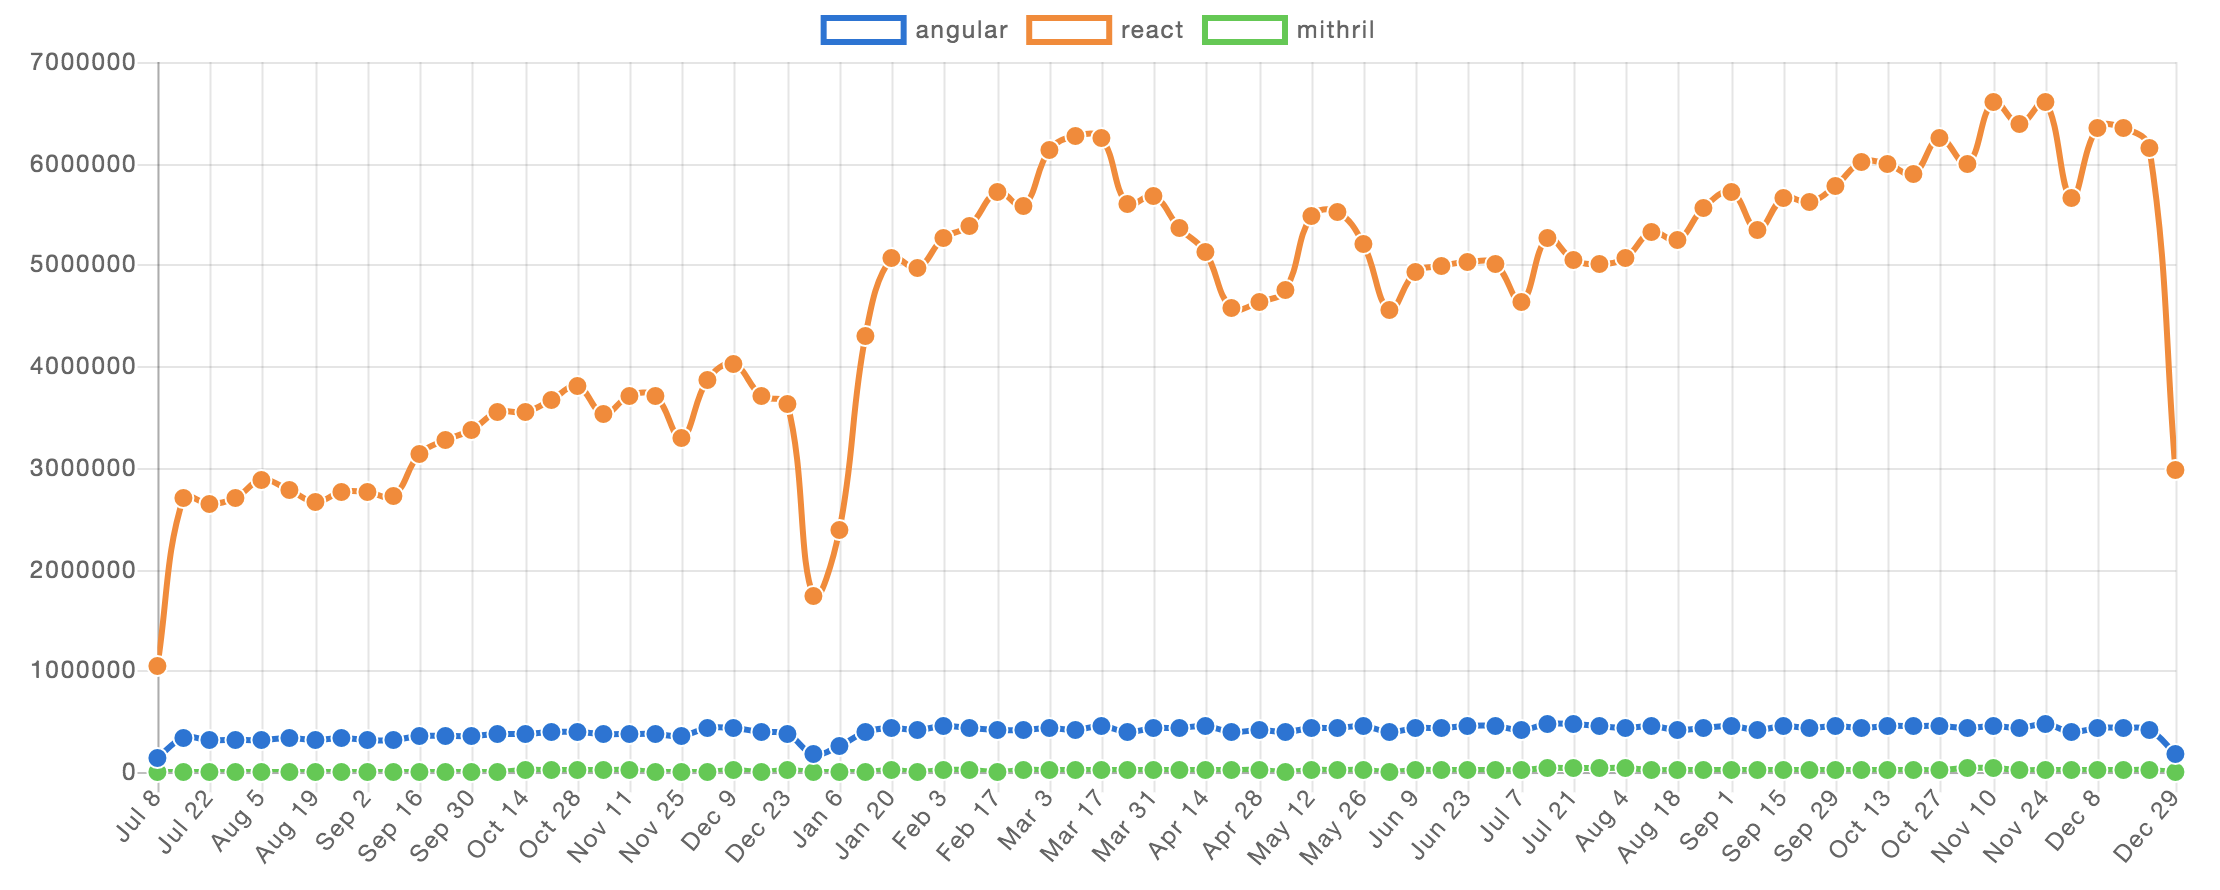
\includegraphics[width=\textwidth]{./img/npmtrends.png}
    \caption{De grafiek in verband met popularteit die gegenereerd werd door npm trends. }
    \label{fig:npmtrends}
\end{figure}

\subsubsection{GitHub statistieken}

Om de populariteit te bepalen kan er ook gekeken worden naar de GitHub statistieken. Deze statistieken geven naast populariteit ook meer inzicht op de problemen die het framework of de bibliotheek heeft en de community er rondom. Deze (afgeronde) statistieken\footnote{bepaald op 5 januari 2020} zijn te zien in tabel \ref{table:github}. Het is duidelijk dat React de meeste fans heeft. Opvallend is dat het aanzienlijk minder problemen heeft dan Angular.

\begin{table}
    \centering
    \begin{tabular}{|c|c|c|c|}
        \cline{2-4}
        \multicolumn{1}{c|}{} & Stars & Forks & Issues \\ \hline
        Angular & 56.0k &  15.4k & 2.8k\\ \hline
        React & 141.8k & 27.2k & 0.7k \\ \hline
        Mithril & 11.9k & 0.9k & 0.1k \\ \hline
        
    \end{tabular}
    \caption{De GitHub statistieken van de drie technologieën. }
    \label{table:github}
\end{table}

\subsubsection{StackOverflow trends}

Ook StackOverflow, een populaire website waar professionals en enthusiastelingen vragen kunnen stellen en waar de community daar dan antwoord op kan geven, heeft een tool waarmee de tendensen vergeleken kunnen worden\footnote{https://insights.stackoverflow.com/trends?tags=angular\%2Creactjs}. Helaas is deze niet volledig, waardoor Mithril niet opgezocht kan worden. Figuur \ref{fig:stackoverflowtrends} toont dan maar de vergelijking tussen Angular en React. 

\begin{figure}
    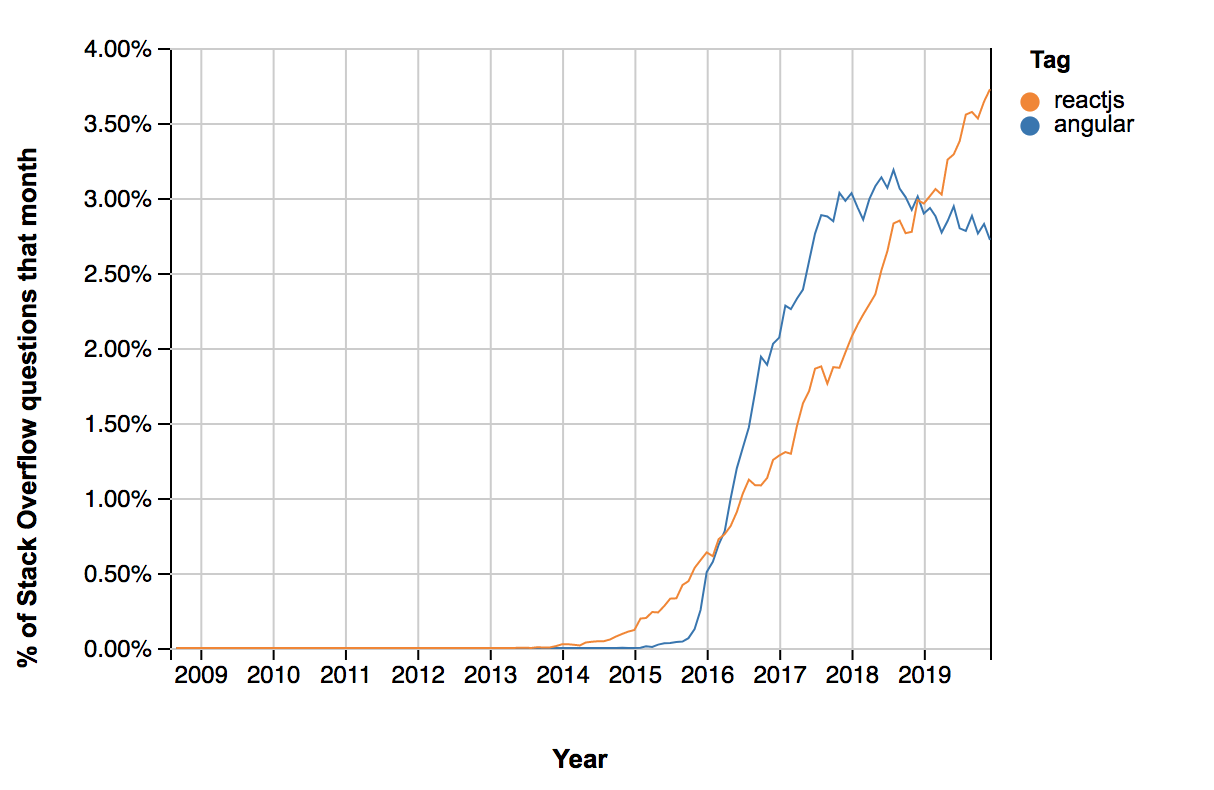
\includegraphics[width=\textwidth]{./img/stackoverflowtrends.png}
    \caption{De grafiek in verband met populariteit die gegenereerd werd door StackOverflow Trends.}
    \label{fig:stackoverflowtrends}
\end{figure}


